\paragraph{Equivariant Policies for Robotic Manipulation}

In imitation learning for robotic manipulation, equivariance has been widely applied to reduce the effort of collecting human demonstrations \citep{zeng2020transporter, huang2022equi-trans, huang2024fourier, ryu2023diffusion, yang2024equibot}. Most prior work focuses on simple pick-and-place tasks, where the policy outputs the 3D pose of the end-effector. By leveraging equivariance, these policies can generalize across different object poses, significantly reducing the number of required demonstrations (e.g., only 5 to 10 demonstrations in \citep{ryu2023diffusion}). However, 3D pose actions are insufficient for tasks that require higher dexterity or involve deformable objects. To address this limitation, Equibot \citep{yang2024equibot} designed an equivariant policy that outputs velocity vectors, achieving success in more complex tasks such as cloth folding and object wrapping. 

There has been limited work on exploiting equivariant policies in reinforcement learning, and existing approaches have largely focused on 2D spaces \citep{wang2022so2equivariant, nguyen2023equivariant}. In this work, we extend the study of equivariant policies to 3D space within a reinforcement learning setting, which, to the best of our knowledge, has not yet been explored for robotic manipulation.
\begin{figure*}[t]
    \makebox[\textwidth][c]{
    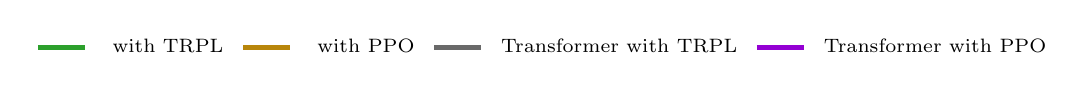
\begin{tikzpicture}
    \tikzstyle{every node}=[font=\scriptsize]
    \definecolor{tabblue}{RGB}{31, 119, 180}
\definecolor{taborange}{RGB}{255, 127, 14}
\definecolor{tabgreen}{RGB}{44, 160, 44}
\definecolor{tabred}{RGB}{214, 39, 40}
\definecolor{tabpurple}{RGB}{148, 103, 189}
\definecolor{tabbrown}{RGB}{140, 86, 75}
\definecolor{tabpink}{RGB}{227, 119, 194}
\definecolor{tabgray}{RGB}{127, 127, 127}
\definecolor{tabolive}{RGB}{188, 189, 34}
\definecolor{tabcyan}{RGB}{23, 190, 207}
\definecolor{lightblue}{RGB}{173, 216, 230}
\definecolor{sandybrown}{RGB}{244, 164, 96}
\definecolor{darkgrey}{RGB}{169, 169, 169}
\definecolor{dimgrey}{RGB}{105, 105, 105}
\definecolor{olivedrab}{RGB}{107, 142, 35}
\definecolor{darkviolet}{RGB}{148, 0, 211}
\definecolor{darkgoldenrod}{RGB}{184, 134, 11}
\definecolor{darkblue}{RGB}{0, 0, 139}
\definecolor{orchid}{RGB}{218, 112, 214}

    \begin{axis}[%
        hide axis,
        xmin=10,
        xmax=50,
        ymin=0,
        ymax=0.1,
        legend style={
            draw=white!15!black,
            legend cell align=left,
            legend columns=4,
            legend style={
                draw=none,
                column sep=1ex,
                line width=1pt,
            }
        },
        ]
        \addlegendimage{line legend, tabgreen, ultra thick} % Thicker line here
        \addlegendentry{\textbf{\model} with TRPL}
        \addlegendimage{line legend, darkgoldenrod, ultra thick} % Thicker line here
        \addlegendentry{\textbf{\model} with PPO}
        \addlegendimage{line legend, dimgrey, ultra thick} % Thicker line here
        \addlegendentry{Transformer with TRPL}
        \addlegendimage{line legend, darkviolet, ultra thick} % Thicker line here
        \addlegendentry{Transformer with PPO}
    \end{axis}
\end{tikzpicture}

    }
    \centering
    \begin{subfigure}[b]{0.32\linewidth}
        \includegraphics[width=\textwidth]{ICLR_2025/Figures/eval_ppo_3_tasks_5_seeds/smooth_eval_ppo_Isaac-Rigid-Insertion-Multi-v0_eval_consistent.pdf}
    \end{subfigure}
    \hfill
    \begin{subfigure}[b]{0.32\linewidth}
        \includegraphics[width=\textwidth]{ICLR_2025/Figures/eval_ppo_3_tasks_5_seeds/smooth_eval_ppo_Isaac-Rope-Shaping-v0_eval_all.pdf}
    \end{subfigure}
    \hfill
    \begin{subfigure}[b]{0.32\linewidth}
        \includegraphics[width=\textwidth]{ICLR_2025/Figures/eval_ppo_3_tasks_5_seeds/smooth_eval_ppo_Isaac-Cloth-Hanging-Multi-v0_eval_all.pdf}
    \end{subfigure}
    
    
    \caption{Performance comparison between HEPi and Transformer models with TRPL and PPO over 10 seeds. TRPL shows stable performance across all tasks, while PPO struggles in tasks requiring high exploration, especially in 3D environments like \textit{cloth-hanging-3D}. In tasks with a lower-dimensional action space (e.g., 2D tasks), both methods perform comparably when carefully tuned.
    % We evaluated each method over 5 seeds, performing a grid search for the best PPO parameters across an additional 5 seeds
    }
    \vspace{-0.2cm}
    \label{fig:eval_trpl_ppo}
\end{figure*}


\paragraph{RL with GNNs}

Graph-based representations in reinforcement learning have shown great success across diverse domains, including molecular design \citep{simm2021symmetryaware}, adaptive mesh refinement \citep{freymuth2023swarm}, and multi-agent systems like traffic light control \citep{pol2022multiagent}. Among these, the most closely related work to ours is morphology reinforcement learning \citep{wang2018nervenet, huang2020smp, pmlr-v162-trabucco22b, hong2022structureaware, gupta2022metamorph}, where the robot’s kinematic structure is represented as a graph, allowing actuators to be controlled through message passing. This approach enables policies to generalize across different robot topologies, particularly in locomotion tasks \citep{gupta2022metamorph}. \citet{chen2023sgrl} extend these ideas to handle 3D environments, but only with sub-equivariant policies for rotations around the gravity axis.

However, these works primarily exploit the locality of graph structures, framing the problem as multi-agent reinforcement learning on graphs \citep{Jiang2020Graph}, where each node can make decisions influenced by its neighbors. In contrast, our work focuses on the underactuated problem where only a small subset of nodes (actuators) controls a much larger set of object nodes, framing a heterogeneous graph. The interactions between the nodes are therefore much more complex to capture using homogeneous GNN models.
